%%%%%%%%%%%%%%%%%%%%%%%%%%%%%%%%%%%%%%%%%%%%%%%%%%%%%%%%%%%%%%%%%%%%%%%%%%%%%
%
%                     Copyright 2010 Jim Finnis.
%                           All Rights Reserved
%
%
%  System        : 
%  Module        : 
%  Object Name   : $RCSfile$
%  Revision      : $Revision$
%  Date          : $Date$
%  Author        : $Author$
%  Created By    : Jim Finnis
%  Created       : Tue Jan 5 19:23:59 2010
%  Last Modified : <110102.1949>
%
%  Description 
%
%  Notes
%
%  History
% 
%%%%%%%%%%%%%%%%%%%%%%%%%%%%%%%%%%%%%%%%%%%%%%%%%%%%%%%%%%%%%%%%%%%%%%%%%%%%%
%
% Copyright (c) 2010 Jim Finnis.
% 
% All Rights Reserved.
% 
% This  document  may  not, in  whole  or in  part, be  copied,  photocopied,
% reproduced,  translated,  or  reduced to any  electronic  medium or machine
% readable form without prior written consent from Jim Finnis.
%
%%%%%%%%%%%%%%%%%%%%%%%%%%%%%%%%%%%%%%%%%%%%%%%%%%%%%%%%%%%%%%%%%%%%%%%%%%%%%

\chapter{Trees and Menus}
\label{trees}
\useglosentry{tree}
\useglosentry{treecol}
As we have already seen, complex collections can contain fields which are
handles to other collections. It's therefore possible to build trees using
collections --- in fact, section \ref{moreiter} contains an example of a sort
of tree built with a collection.

SCMS' Tag Definition Language doesn't\footnote{yet} have the syntax to create
these trees easily yourself, although it's easy to create them from inside
PHP\footnote{see Chapter \ref{collimp}: Collection Implementation}. It does,
however, provide two very useful `built in' trees: the navigation tree and the
language tree\footnote{As we'll see later, the language tree isn't really a
tree since it only has one level, but it does have the selection properties of
a tree and so uses tree code.}. It also provides powerful mechanisms for
walking and otherwise navigating a tree hierarchy.

\section{Tree handles}
In the same way as collections are referenced by collection handles, trees are
referenced by \emph{tree handles}. Trees are effectively a subclass of
collections: a tree handle is also a collection handle, and can be used as
such, but a collection handle cannot be used in any of the tags which are for
tree handles only. Tree handles are strings of the form \texttt{tree:$n$}.

\section{Structure of a tree node}
\useglosentry{node}
Trees in SCMS are a little unusual, because the fundamental concept they are
built around is not a tree node, but a collection of nodes. For instance, the
root level of the tree is a collection which (as we already know) is made up
of an array of items. Some of these items have children, which are also
collections.

From a nomenclature standpoint, I'll use the word \emph{node} to refer to what
in a collection is normally referred to as an \emph{item}. They're
fundamentally the same thing, but a node is part of a tree rather than a plain
\indtag{collection item tags!child}
collection, and always has a \texttt{child} field (and a few others as
specified below).

If a node has an empty string for the child field, or it is unset, the node
doesn't have a child tree. If it does have children, the \texttt{child} field
will hold the tree handle for the subtree. Tree collections differ from normal
collections in that they also contain a handle to the parent collection
\indtag{tree item fields!parentc}
(called \texttt{parentc},) and the index number of the parent node within that
\indtag{tree item fields!parenti}
collection (called \texttt{parenti}.) Note that these are not fields within
nodes: they are properties of a tree collection as a whole, and there are
special tags for accessing them.

\begin{figure}[htp]
\centering
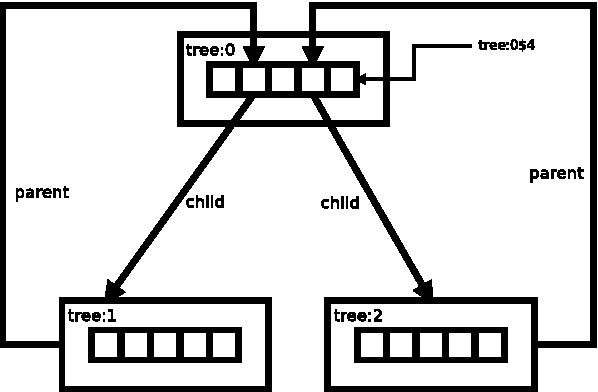
\includegraphics[width=3in]{tree.pdf}
\caption{Tree structure}
\label{fig1}
\end{figure}
Figure~\ref{fig1} shows three tree collections making up a two level tree. The
collection with handle \texttt{tree:0} is the root. Collection \texttt{tree:1}
is the child of the second node in \texttt{tree:0}, while \texttt{tree:2} is
the child of the fourth node. We've also shown a \emph{node handle}, which
points to the fifth node in \texttt{tree:0}. This will come in handy later
when we need a single entity to refer to a single node in a tree. \clearpage
\noindent In terms of field values, this means that:
\begin{itemize}
\item The \texttt{child} field of node 1\footnote{i.e. the second node: all indices are zero based} in \texttt{tree:0}
has the string value \texttt{tree:1}.
\item The \texttt{child} field of node 3 in \texttt{tree:0} has the string value \texttt{tree:2}.
\item The \texttt{child} fields of all the other nodes are either unset or zero length strings.
\item Collection \texttt{tree:1} has a \texttt{parentc} of \texttt{tree:0} and a \texttt{parenti} of 1.
\item Collection \texttt{tree:2} has a \texttt{parentc} of \texttt{tree:0} and a \texttt{parenti} of 3.
\item Collection \texttt{tree:0} has an unset or zero length \texttt{parentc} value, because it is the root.
\end{itemize}

\subsection{Other fields}
As well as the \texttt{child} field, items (nodes) in a tree collection
contain the all the fields of a collection item and some extra fields:
\begin{itemize}
\indtag{tree item fields!ishome}
\item \texttt{ishome} is nonzero if the node is the first in the root level.
\indtag{tree item fields!isintrail}
\useglosentry{trail}
\item \texttt{isintrail} is true if the node is in the trail down to the selected node after a \texttt{marktree} (see below).
\indtag{tree item fields!issel}
\item \texttt{issel} is true if the node is the selected node after a \texttt{marktree} (see below).
\indtag{tree item fields!index}
\item \texttt{index} is the index of the current node within the current collection. It's
not actually a field, being set dynamically during the render, but it behaves
like one.
\indtag{tree item fields!level}
\item \texttt{level} is the level of the current node within the current collection. Like \texttt{index}, it's
not actually a field.
\indtag{tree item fields!handle}
\item \texttt{handle} is the node handle of the current node within the current collection. Another `pseudofield.'
\end{itemize}

\section{The navigation tree}
\useglosentry{navfile}
\useglosentry{navtree}
This tree is created from the \texttt{site/navigation} file, whose format is
fully explained in Chapter \ref{navig}: Navigation. Briefly, it describes a
hierarchy of pages which can have more than one root (although the first page
at the top level is always the home page) using hyphens to show indent level:
\begin{MyVerbatim}
home
-page1
-page2
--page22
--page23
-other/page3
other/help
\end{MyVerbatim}
Here, we can see that the two pages \texttt{home} and \texttt{other/help} are
at the top, root level; while pages \texttt{page1}, \texttt{page2} and
\texttt{other/page3} are under the \texttt{home} page. Finally, \texttt{page2}
contains two pages: \texttt{page22} and \texttt{page23}. The names are the
page specifiers --- i.e. the files under \texttt{site/pages} which contain the
page's data. Note, as we pointed out in the Pages chapter, the hierarchy we
are specifying here is \emph{not the same} as the file structure!

\indtag{navtree}
The navigation tree's handle can be obtained from the \texttt{navtree} tag.
Since a tree is essentially a collection, we can iterate over the top level
with \texttt{foreach}:
\begin{MyVerbatim}
{{foreach|{{navtree}}|node|
    {{node:name}}<br>
    }}
\end{MyVerbatim}
We'll just get the page names for \texttt{home} and \texttt{other/help}
written out, since \texttt{foreach} doesn't know how to walk a full tree.

\subsection{Additional fields}
As well as the default tree fields listed above, nodes in the navigation tree also have the following fields:
\begin{itemize}
\indtag{navigation tree node fields!spec}
\item \texttt{spec} is the page specifier of the page, as listed in the \texttt{site/navigation} file.
\indtag{navigation tree node fields!url}
\item \texttt{url} is the URL of the page.
\indtag{navigation tree node fields!name}
\item \texttt{name} is the name of the page, as taken from the \texttt{page:name} tag.
\indtag{navigation tree node fields!type}
\item \texttt{type} is the type of the page, a single letter with values 'N' for normal, 'I' for invisible,
and 'H' for heading only. These are set using special punctuation in the navigation menu -- see Chapter \ref{navig}: Navigation
for more details.
\end{itemize}

\subsection{Loading and Caching}
The navigation tree is created when it's first requested. It's actually
cached, held in the \texttt{tmp} directory with a separate file for each
language. This is to avoid a lot of page file reads for large sites: if we
created the navigation tree afresh on each run we'd have to load in every page
file to get the \texttt{page:name} values. However, you shouldn't usually need
to worry about this because if the file doesn't exist, or is old, it will
automatically be rebuilt. If there is a problem, you may want to consider
running the \texttt{clearcache} script from your site's root directory. This
will delete the cached files.

\section{Marking the tree}
\label{treemark}
\useglosentry{trail}
Once you've loaded or created a tree, such as the navigation tree, you'll
probably need to mark the currently selected node and all those nodes in the
trail down from the root to the selected one. To do this, we use the
\indtag{marktree}
\texttt{marktree} tag. You need to have the tree handle, the name of a field
giving a unique ID for each node, and the value of that field in the selected
node. In the navigation menu, the unique ID is the \texttt{spec} field (the
page specifier); and the value of that field in the selected node will be the
current page's page specifier, which is returned from the \texttt{spec} tag:
\begin{MyVerbatim}
{{marktree|{{navtree}}|spec|{{spec}}}}
\end{MyVerbatim}
The \texttt{marktree} tag itself produces no output, it just clears any
marking on the tree and then walks it, setting the appopriate fields in the
nodes.

\clearpage
\section{Rendering a tree}
\label{treerender}
\useglosentry{noderentemp}
To output a tree into your page, you need to walk the tree using the
\texttt{rendertree} tag. Before you do that, however, you need to use various tags
to define the \emph{node rendering templates}
which set how the tree should be rendered. These tags output no data
themselves. The tags you'll need to use are:
\begin{itemize}
\indtag{treeprefix}
 \item \verb,{{treeprefix|level|prefix}}, sets a string to put before starting a new tree or a new level of a
 multilevel tree. For example, this might be a \texttt{<ul>} tag to open a list of nodes. See below for
 information on levels, but the `level' value is often \texttt{default}, indicating that the same string is to be used for
 all levels.
\indtag{treesuffix}
\item \verb,{{treesuffix|level|suffix}}, similarly sets a string to render after a particular tree or subtree,
 such as \texttt{</ul>}.
\indtag{treeunselnode}
\item \verb,{{treeunselnode|level|strpre|strpost}}, sets two template strings to use to render each unselected tree
 node. Again,
 this can be set differently for each level of the tree. The templates will make use of the the fields 
 in the tree nodes, prefixed with the prefix set in \texttt{rendertree}. The `strpre' string will be used 
 before any subtrees are rendered, and the `strpost' string will appear after them. You can think of the
 pre and post strings as a single string, broken in two. Any subtree output is inserted between the two.
\indtag{treetrailnode}
\item \verb,{{treetrailnode|level|strpre|strpost}}, sets template strings to use to render nodes marked
as being in the trail from the root down to the selected node.
\indtag{treeselnode}
\item \verb,{{treeselnode|level|strpre|strpost}}, sets template strings to use to render the selected node.
\end{itemize}

\clearpage
Once these tags are all set up, you can render the tree using the
\indtag{rendertree}
\texttt{{rendertree}} tag. This takes two arguments: the tree handle, and the
prefix for the node field tags in the templates. Here's an example:

\begin{MyVerbatim}
## Each level of the menu is an HTML unordered list,
## and so has <ul>.. </ul> around it.

{{treeprefix|default|<ul>}}
{{treesuffix|default|</ul>}}

## unselected nodes are rendered as list items containing
## a link to the named page

{{treeunselnode|default|
    <li><a href="{{a:url}}"{{a:name}}</a>|</li>
    ##         subtrees output goes here ^
}}

## trail nodes have links, but in bold

{{treetrailnode|default|
    <li><b><a href="{{a:url}}"{{a:name}}</a></b>|</li>
}}

## the selected node is rendered as just the name,
## since there's no point having a link to a page
## you're on.

{{treeselnode|default|
    <li>{{a:name}}|</li>
}}


## Now we can render the tree.

{{rendertree|{{navtree}}|a}}
\end{MyVerbatim}

\clearpage
\subsection{If node selection templates are undefined}
\label{unspectreetemps}
If you haven't used one of \texttt{treeunselnode}, \texttt{treeselnode} or
\texttt{treetrailnode} for the current tree the system will fall back to
templates you have defined, using the following rules:
\begin{itemize}
\item If \texttt{treeselnode} is not defined, the system will try to use \texttt{treetrailnode}. If that's
not defined either, it will try to use \texttt{treeunselnode}.
\item If \texttt{treetrailnode} is not defined, it will first try \texttt{treeunselnode}, then \texttt{treeselnode}.
\item If \texttt{treeunselnode} is not defined, it will first try \texttt{treetrailnode}, then \texttt{treeselnode}.
\end{itemize}

You can find a more complex example of all of these tags in use in Chapter~\ref{navig}, Navigation.

\subsection{Automatic clearing}
Note that all the tree rendering templates are immediately cleared
after \texttt{rendertree} is called.

\subsection{Levels}
As noted above, the five template setting tags take a level argument, which is
\texttt{default} in all our examples. This argument can allow each level of
the menu to be rendered using a different style. The level is a number
starting at zero for the root level, or the word \texttt{default} which
indicates that we are defining a template for use in levels where no specific
level template has been defined. Here's an example:
\begin{MyVerbatim}
 {{treeprefix|0|<ul class="toplevel">}}
 {{treeprefix|1|<ul class="2ndlevel">}}
 {{treesuffix|default|</ul>}}
\end{MyVerbatim}
This will make the top level of the tree render using the CSS class
\texttt{toplevel}, and the second level render with the class
\texttt{2ndlevel}. The suffix for both levels of the menu will be the same,
because \texttt{default} was specified.

\clearpage
\section{Navigating the tree}
\label{treenav}
It's sometimes useful to navigate the tree in more complex ways, and there are
tags to allow this.

\subsection{Setting temporary collection tags}
\label{colltags}
You may find that you need to store a collection handle in a tag, and then get fields from this tag
using the syntax in sections \ref{collbyindex} and \ref{collbyindex2}. You might be tempted to
do something like this:
\begin{MyVerbatim}
## get the child collection of the first node in the
## navtree
{{set|foo|{{navtree|0|child}}}}

## print the name of its first node
{{foo|0|name}}
\end{MyVerbatim}
This won't work -- \texttt{foo} is a tag name, not a tree handle. However, you know that it \emph{contains}
a tree name, so you might be tempted to try
\begin{MyVerbatim}
{{{{foo}}|0|name}}
\end{MyVerbatim}
This still won't work: you can't use \verb,{{foo}}, as the name of a tag because tag names aren't processed
through the templater. It wouldn't help even if they were, because you'd be trying to use a tree handle
as if it were a tag name; they're two completely different namespaces.

What you can do is create a \emph{collection tag}. In the same way as when you created collections
in Chapter~\ref{collchap}, you can create a new tag which contains a collection handle, and which the
templater knows contains a collection handle rather than just a string. You can do this using the
\texttt{setcoll} tag:
\indtag{setcoll}
\begin{MyVerbatim}
## get the child collection of the first node in the
## navtree and store it in a collection tag
{{setcoll|foo|{{navtree|0|child}}}}

## print the name of its first node
{{foo|0|name}}
\end{MyVerbatim}
This will now work, because SCMS knows that \texttt{foo} refers to a collection.

\subsection{Finding the parent tree collection of a node}
\indtag{findcollection}
The tag \texttt{findcollection} can, given a field name and a value, search a tree for a given node. It
will then return the tree handle of the collection which contains that node, so it can be walked
with \texttt{foreach}, \texttt{rendertree}
and so on. Syntactically it's very like \texttt{marktree} --- so to find the collection containing
the current page in the navigation tree, you would use
\begin{MyVerbatim}
{{findcollection|spec|{{spec}}}}
\end{MyVerbatim}

\subsection{Finding the parent node of a tree collection}
\indtag{parentc}
\indtag{parenti}
To find the parent node of a collection given the collection handle, there are two tags:
\texttt{parentc} will return the collection handle of the parent, and \texttt{parenti} will return
 the parent node index within that collection:
\begin{MyVerbatim}
## set a temporary tag, tmp, to the collection
## the current page is in
{{setcoll|tmp|
    {{findcollection|{{navtree}}|spec|{{spec}}}}}}

## set a tag, pc,  to contain the handle
## for the parent collection of the collection
## in tmp
{{setcoll|pc|{{parentc|{{tmp}}}}}}

## and set pi to contain the index of tmp in
## that parent collection
{{set|pi|{{parenti|{{tmp}}}}}}

## Now show the name of that node, if the parent
## collection is not null
{{ifnotempty|{{pc}}|
    {{pc|{{pi}}|name}}
    |No parent node
}}f
\end{MyVerbatim}
This will get the collection the current page's is in, find the parent node of that node, and show its name.
In other words, it will show the name of the parent page in a hierarchical navigation structure. It's a
little long-winded, so there's a better way to do it using \emph{node handles}.

\subsection{Node handles}
A node handle is a tree handle with a suffix referencing a node in the tree collection. Take a look
at the diagram at the start of this chapter. You'll see that the fifth node in the collection
\texttt{tree:0} has the handle \texttt{tree:0\$4}. The handle consists of the tree handle, followed by a
dollar sign, followed by the node's index.

\subsection{Finding a node}
\indtag{findnode}
Without node handles, we couldn't represent nodes by a single value and so had no way of searching for a
node in the tree. The best we could do was use \texttt{findcollection} to find the collection
which contained that node. Now we can do better, using \texttt{findnode}. This has the same arguments ---
field to search and search string --- but returns the node handle of the node in which the given field
equals the given string:
\begin{MyVerbatim}
## print the node handle of the current page's
## node in the navigation tree
{{findnode|{{navtree}}|spec|{{spec}}}}
\end{MyVerbatim}
Incidentally, while you can do this --- search for the current node in the navigation tree using
\texttt{findnode} --- the navigation menu system has a shortcut: \usetag{curnavnode} contains
a handle to the current page's node in the navigation tree.

\subsection{Finding the handle of the parent node of a node or tree}
\indtag{parent}
The \texttt{parent} tag, which takes either a tree handle or a node handle,
returns the node handle of the parent:
\begin{MyVerbatim}
## find the node, setting a temporary
{{set|tmp|
    {{findnode|{{navtree}}|spec|{{spec}}}}}}

## print out the handle of the parent if there is one.
## Otherwise, an empty string.
{{parent|{{tmp}}}}
\end{MyVerbatim}
\clearpage
\subsection{Using node handles in place of tree handles}
\indtagsec{findnode}
The last tag illustrates a general principle: you can use a node handle anywhere you 
can use a tree or collection handle, and it will act as the handle for the tree or collection
which contains that node. For example, this will iterate over the nodes at the same level
in the tree as the current page:
\begin{MyVerbatim}
{{foreach|{{findnode|{{navtree}}|spec|{{spec}}}}|a|
    {{a:name}}
}}
\end{MyVerbatim}
Those of you with your eyes on the ball will note that this principle of being able to use
node handles where tree handles can be used, when combined with \texttt{findnode}, means that
\texttt{findcollection} is redundant. It's left in mainly to illustrate the usage of \texttt{parentc}
and \texttt{parenti}, and for legacy templates.

\subsection{Using fields in the node handle}
As yet we can't do much with the node handle itself; we'll now see how to access the fields in
a node represented by a node handle. There are several different ways to do this.

\subsubsection{Using \texttt{getfield} to directly get the field values}
\label{fieldget}
\indtag{getfield}
The simplest way is to use the \texttt{getfield}
tag, which takes the node handle and the name of a field:
\begin{MyVerbatim}
{{set|tmp|
    {{findnode|{{navtree}}|spec|{{spec}}}}}}

{{getfield|{{tmp}}|name}}
\end{MyVerbatim}
This will print the name of the current page; a little pointless given that it's just the same
as doing \verb,{{spec}},.

Also, if the node handle is stored with the correct type using \texttt{setnode} (see below),
you can use the field name as an argument:
\begin{MyVerbatim}
{{setnode|tmp|
    {{findnode|{{navtree}}|spec|{{spec}}}}}}

{{tmp|name}}
\end{MyVerbatim}

\subsubsection{Creating temporary node tags with setnode}
\label{usenodetag}
\indtag{setnode}
\indtag{setitem}
Alternatively, we can use a similar system to the collection tags in section~\ref{colltags} above, and
create a temporary \emph{node tag}. We can do this by using the \texttt{setnode} function tag instead
of a plain \texttt{set}:
\begin{MyVerbatim}
{{setnode|tmp|
    {{findnode|{{navtree}}|spec|{{spec}}}}}}

## use the node tag
{{p|name}}
\end{MyVerbatim}
The tag \texttt{setitem} is also available; it is just an alternative name for \texttt{setnode}.

\subsubsection{Using \texttt{withnode} to access fields}
\indtag{withnode}
Finally, it's possible to use the \texttt{withnode} tag. This takes a node handle, a tag name prefix,
and a template, and defines all the tags with the values of all the fields in the node and runs
the template with those tag definitions. In other words, it works rather like \texttt{foreach} but for
a single node:
\begin{MyVerbatim}
{{withnode|{{findnode|{{navtree}}|spec|{{spec}}}}|a|
    {{a:name}} has the url {{a:url}}
}}
\end{MyVerbatim}

\subsection{Finding the parent collection of a node}
Note that this doesn't mean the collection a node is in --- since node handles can be used where
tree handles are used, we can just use the node handle itself for that. The `parent collection' here means
the tree collection which \emph{contains} the tree collection the node is in.
Again, since node handles can be used where tree handles are accepted, we can use the \texttt{parentc}
tag to find the parent collection of a node. We can therefore iterate over all the nodes in the
level above a given node using:
\begin{MyVerbatim}
## find the current page's node
{{setnode|tmp|
    {{findnode|{{navtree}}|spec|{{spec}}}}}}
    
## find the parent collection of the
## collection that node is in
{{setnode|tmp|{{parentc|{{tmp}}}}}}    

## if it's not empty (i.e. we weren't at root)
## iterate over it
{{ifnotempty|{{tmp}}|
    {{foreach|{{tmp}}|a|
        {{a:name}}
    }}
|}}
\end{MyVerbatim}

\subsection{Finding the index of a node}
\indtag{indexof}
To do this, just use the \texttt{indexof} tag with the node handle:
\begin{MyVerbatim}
{{setnode|tmp|
    {{findnode|{{navtree}}|spec|{{spec}}}}}}

I am number {{indexof|{{tmp}}}} in my level.
\end{MyVerbatim}

\subsection{Node handles in iterators}
As well as setting the fields and the \texttt{index} and \texttt{level} values etc.,
iterators like \texttt{foreach} and \texttt{rendertree} will also set a \texttt{handle}
value which contains the node handle of the node currently being output:
\begin{MyVerbatim}
{{foreach|{{navtree}}|a|
## a:handle is defined as a node tag, so
    {{a:handle|name}}
## is the same as
    {{a:name}}
}}
\end{MyVerbatim}

\subsection{Finding the child of a node}
If a node has a child, its \texttt{child} field will contain the tree handle
of the child subtree. You could, therefore, iterate over the top two levels
of the navigation tree producing a cartesian product using:
\begin{MyVerbatim}
{{foreach|{{navtree}}|a|
   {{ifnotempty|{{a:child}}|
       {{foreach|{{a:child}}|b|
            {{a:name}}/{{b:name}}}}
   |}}
}}
\end{MyVerbatim}

\subsection{Checking whether a field is set}
\indtag{iffieldset}
The above code could also be written in the following way, using \texttt{iffieldset} to test if there is
a child:
\begin{MyVerbatim}
{{foreach|{{navtree}}|a|
   {{iffieldset|{{a:handle}}|child|
       {{foreach|{{a:child}}|b|
            {{a:name}}/{{b:name}}}}
   |}}
}}
\end{MyVerbatim}


